% Options for packages loaded elsewhere
\PassOptionsToPackage{unicode}{hyperref}
\PassOptionsToPackage{hyphens}{url}
%
\documentclass[
  oneside]{book}
\usepackage{amsmath,amssymb}
\usepackage{iftex}
\ifPDFTeX
  \usepackage[T1]{fontenc}
  \usepackage[utf8]{inputenc}
  \usepackage{textcomp} % provide euro and other symbols
\else % if luatex or xetex
  \usepackage{unicode-math} % this also loads fontspec
  \defaultfontfeatures{Scale=MatchLowercase}
  \defaultfontfeatures[\rmfamily]{Ligatures=TeX,Scale=1}
\fi
\usepackage{lmodern}
\ifPDFTeX\else
  % xetex/luatex font selection
\fi
% Use upquote if available, for straight quotes in verbatim environments
\IfFileExists{upquote.sty}{\usepackage{upquote}}{}
\IfFileExists{microtype.sty}{% use microtype if available
  \usepackage[]{microtype}
  \UseMicrotypeSet[protrusion]{basicmath} % disable protrusion for tt fonts
}{}
\makeatletter
\@ifundefined{KOMAClassName}{% if non-KOMA class
  \IfFileExists{parskip.sty}{%
    \usepackage{parskip}
  }{% else
    \setlength{\parindent}{0pt}
    \setlength{\parskip}{6pt plus 2pt minus 1pt}}
}{% if KOMA class
  \KOMAoptions{parskip=half}}
\makeatother
\usepackage{xcolor}
\usepackage{color}
\usepackage{fancyvrb}
\newcommand{\VerbBar}{|}
\newcommand{\VERB}{\Verb[commandchars=\\\{\}]}
\DefineVerbatimEnvironment{Highlighting}{Verbatim}{commandchars=\\\{\}}
% Add ',fontsize=\small' for more characters per line
\usepackage{framed}
\definecolor{shadecolor}{RGB}{248,248,248}
\newenvironment{Shaded}{\begin{snugshade}}{\end{snugshade}}
\newcommand{\AlertTok}[1]{\textcolor[rgb]{0.94,0.16,0.16}{#1}}
\newcommand{\AnnotationTok}[1]{\textcolor[rgb]{0.56,0.35,0.01}{\textbf{\textit{#1}}}}
\newcommand{\AttributeTok}[1]{\textcolor[rgb]{0.13,0.29,0.53}{#1}}
\newcommand{\BaseNTok}[1]{\textcolor[rgb]{0.00,0.00,0.81}{#1}}
\newcommand{\BuiltInTok}[1]{#1}
\newcommand{\CharTok}[1]{\textcolor[rgb]{0.31,0.60,0.02}{#1}}
\newcommand{\CommentTok}[1]{\textcolor[rgb]{0.56,0.35,0.01}{\textit{#1}}}
\newcommand{\CommentVarTok}[1]{\textcolor[rgb]{0.56,0.35,0.01}{\textbf{\textit{#1}}}}
\newcommand{\ConstantTok}[1]{\textcolor[rgb]{0.56,0.35,0.01}{#1}}
\newcommand{\ControlFlowTok}[1]{\textcolor[rgb]{0.13,0.29,0.53}{\textbf{#1}}}
\newcommand{\DataTypeTok}[1]{\textcolor[rgb]{0.13,0.29,0.53}{#1}}
\newcommand{\DecValTok}[1]{\textcolor[rgb]{0.00,0.00,0.81}{#1}}
\newcommand{\DocumentationTok}[1]{\textcolor[rgb]{0.56,0.35,0.01}{\textbf{\textit{#1}}}}
\newcommand{\ErrorTok}[1]{\textcolor[rgb]{0.64,0.00,0.00}{\textbf{#1}}}
\newcommand{\ExtensionTok}[1]{#1}
\newcommand{\FloatTok}[1]{\textcolor[rgb]{0.00,0.00,0.81}{#1}}
\newcommand{\FunctionTok}[1]{\textcolor[rgb]{0.13,0.29,0.53}{\textbf{#1}}}
\newcommand{\ImportTok}[1]{#1}
\newcommand{\InformationTok}[1]{\textcolor[rgb]{0.56,0.35,0.01}{\textbf{\textit{#1}}}}
\newcommand{\KeywordTok}[1]{\textcolor[rgb]{0.13,0.29,0.53}{\textbf{#1}}}
\newcommand{\NormalTok}[1]{#1}
\newcommand{\OperatorTok}[1]{\textcolor[rgb]{0.81,0.36,0.00}{\textbf{#1}}}
\newcommand{\OtherTok}[1]{\textcolor[rgb]{0.56,0.35,0.01}{#1}}
\newcommand{\PreprocessorTok}[1]{\textcolor[rgb]{0.56,0.35,0.01}{\textit{#1}}}
\newcommand{\RegionMarkerTok}[1]{#1}
\newcommand{\SpecialCharTok}[1]{\textcolor[rgb]{0.81,0.36,0.00}{\textbf{#1}}}
\newcommand{\SpecialStringTok}[1]{\textcolor[rgb]{0.31,0.60,0.02}{#1}}
\newcommand{\StringTok}[1]{\textcolor[rgb]{0.31,0.60,0.02}{#1}}
\newcommand{\VariableTok}[1]{\textcolor[rgb]{0.00,0.00,0.00}{#1}}
\newcommand{\VerbatimStringTok}[1]{\textcolor[rgb]{0.31,0.60,0.02}{#1}}
\newcommand{\WarningTok}[1]{\textcolor[rgb]{0.56,0.35,0.01}{\textbf{\textit{#1}}}}
\usepackage{longtable,booktabs,array}
\usepackage{calc} % for calculating minipage widths
% Correct order of tables after \paragraph or \subparagraph
\usepackage{etoolbox}
\makeatletter
\patchcmd\longtable{\par}{\if@noskipsec\mbox{}\fi\par}{}{}
\makeatother
% Allow footnotes in longtable head/foot
\IfFileExists{footnotehyper.sty}{\usepackage{footnotehyper}}{\usepackage{footnote}}
\makesavenoteenv{longtable}
\usepackage{graphicx}
\makeatletter
\def\maxwidth{\ifdim\Gin@nat@width>\linewidth\linewidth\else\Gin@nat@width\fi}
\def\maxheight{\ifdim\Gin@nat@height>\textheight\textheight\else\Gin@nat@height\fi}
\makeatother
% Scale images if necessary, so that they will not overflow the page
% margins by default, and it is still possible to overwrite the defaults
% using explicit options in \includegraphics[width, height, ...]{}
\setkeys{Gin}{width=\maxwidth,height=\maxheight,keepaspectratio}
% Set default figure placement to htbp
\makeatletter
\def\fps@figure{htbp}
\makeatother
\setlength{\emergencystretch}{3em} % prevent overfull lines
\providecommand{\tightlist}{%
  \setlength{\itemsep}{0pt}\setlength{\parskip}{0pt}}
\setcounter{secnumdepth}{-\maxdimen} % remove section numbering
\newlength{\cslhangindent}
\setlength{\cslhangindent}{1.5em}
\newlength{\csllabelwidth}
\setlength{\csllabelwidth}{3em}
\newlength{\cslentryspacingunit} % times entry-spacing
\setlength{\cslentryspacingunit}{\parskip}
\newenvironment{CSLReferences}[2] % #1 hanging-ident, #2 entry spacing
 {% don't indent paragraphs
  \setlength{\parindent}{0pt}
  % turn on hanging indent if param 1 is 1
  \ifodd #1
  \let\oldpar\par
  \def\par{\hangindent=\cslhangindent\oldpar}
  \fi
  % set entry spacing
  \setlength{\parskip}{#2\cslentryspacingunit}
 }%
 {}
\usepackage{calc}
\newcommand{\CSLBlock}[1]{#1\hfill\break}
\newcommand{\CSLLeftMargin}[1]{\parbox[t]{\csllabelwidth}{#1}}
\newcommand{\CSLRightInline}[1]{\parbox[t]{\linewidth - \csllabelwidth}{#1}\break}
\newcommand{\CSLIndent}[1]{\hspace{\cslhangindent}#1}
\ifLuaTeX
\usepackage[bidi=basic]{babel}
\else
\usepackage[bidi=default]{babel}
\fi
\babelprovide[main,import]{spanish}
% get rid of language-specific shorthands (see #6817):
\let\LanguageShortHands\languageshorthands
\def\languageshorthands#1{}
\usepackage{makeidx}
\makeindex
\usepackage{graphicx}
\usepackage{tikz}
\usepackage{atbegshi}


\AtBeginDocument{
    \AtBeginShipoutNext{
        \AtBeginShipoutUpperLeft{
            \put(\dimexpr\paperwidth/2-\textwidth/2\relax, -650){
                \makebox[\textwidth]{
                    
\includegraphics[width=0.45\textwidth]{cure_udelar.png}  % Adjust width as needed
                    \hfill
                    
\includegraphics[width=0.405\textwidth]{logoMEDIA.jpeg} % Make it 90% smaller
                }
            }
        }
    }
}
\ifLuaTeX
  \usepackage{selnolig}  % disable illegal ligatures
\fi
\IfFileExists{bookmark.sty}{\usepackage{bookmark}}{\usepackage{hyperref}}
\IfFileExists{xurl.sty}{\usepackage{xurl}}{} % add URL line breaks if available
\urlstyle{same}
\hypersetup{
  pdftitle={Entrega: curso de datos extremales},
  pdfauthor={Laura Montaldo, CI: 3.512.962-7},
  pdflang={es},
  hidelinks,
  pdfcreator={LaTeX via pandoc}}

\title{Entrega: curso de datos extremales}
\author{Laura Montaldo, CI: 3.512.962-7}
\date{2024-02-26}

\begin{document}
\frontmatter
\maketitle

\mainmatter
\newpage

\thispagestyle{empty}

\maketitle

\newpage

\tableofcontents

\newpage

\hypertarget{resumen}{%
\chapter{Resumen}\label{resumen}}

Your abstract goes here.

\newpage

\chapter{Motivación y objetivo del estudio}

Los índices de \(S\&P\) son una familia de índices de renta
variable\footnote{En inglés se llaman equity indices} diseñados para
medir el rendimiento del mercado de acciones en Estados Unidos que
cotizan en bolsas estadounidenses. Ésta familia de índices está
compuesta por una amplia variedad de índices basados en tamaño, sector y
estilo. Los índices están ponderados por el criterio
\textit{float-adjusted market capitalization} (FMC). Además, se disponen
de índices ponderados de manera equitativa y con límite de
capitalización de mercado, como es el caso del \(S\&P\:500\). Este este
sentido, el \(S\&P 500\) entraría en el conjunto de índices ponderados
por capitalización bursátil ajustada a la flotación (ver
\href{http://www.overleaf.com}{\textcolor{blue}{$S\&P$ Dow Jones Indices}}).
El mismo mide el rendimiento del segmento de gran capitalización del
mercado estadounidense. Es considerado como un indicador representativo
del mercado de renta variable de los Estados Unidos, y está compuesto
por 500 empresas constituyentes.

Se busca crear un indicador de una posible crisis bursátil. Como
variable de referencia de toma la relación de precios al cierre de ayer
sobre la de hoy

\begin{equation}
Indicador_t=\frac{Precio_{t-1}}{Precio_t},\quad\text{para}\; t=1,...,T \label{eq:ind}
\end{equation} \vspace{0.5cm}

Interpretación del Indicador:

\begin{itemize}
\item Si el $Indicador_t$    $\leq$ 1, el precio de cierre de hoy es mayor o igual que el de ayer, lo cual podría ser considerado una señal positiva.
\item Si el $Indicador_t$ > 1, el precio de cierre de hoy es menor que el de ayer, lo cual podría considerarse una señal de alerta.
\end{itemize}

\vspace{1cm}

En las siguiente figura @ref(fig:plot1) se muestra la evolución
histórica desde la fecha 03/01/1928 hasta 08/12/2023 del precio al
cierre del día del indicar S\&P 500.

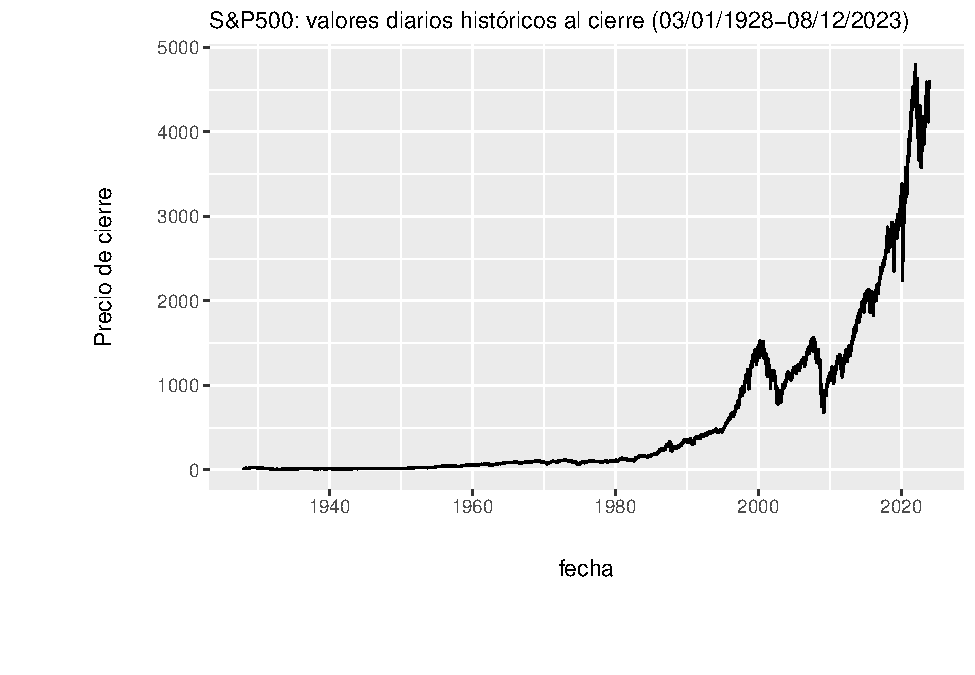
\includegraphics{extremales_files/figure-latex/plot1-1.pdf}

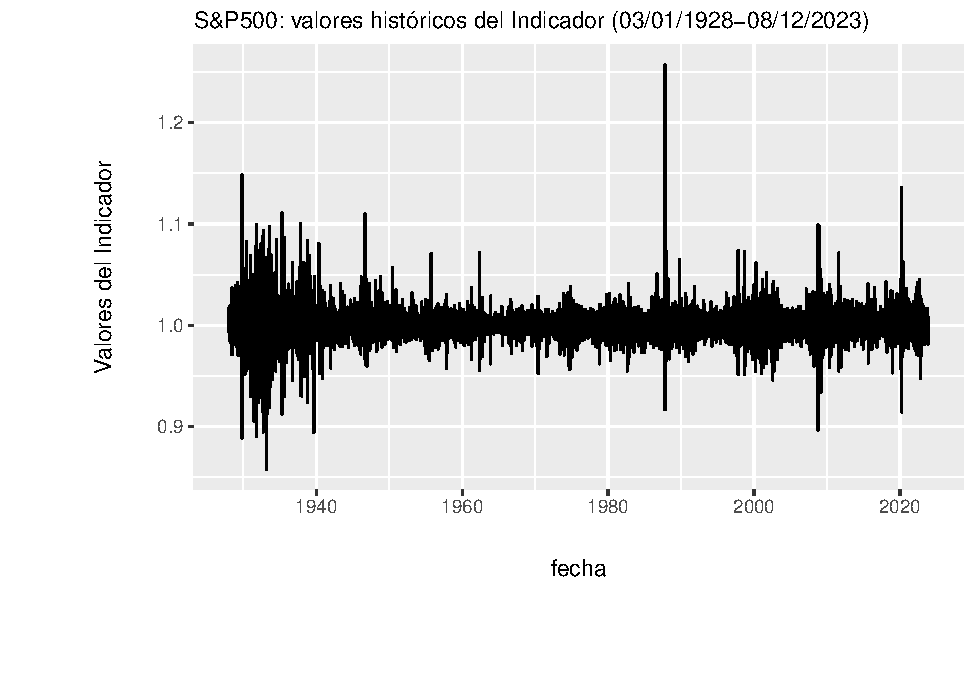
\includegraphics{extremales_files/figure-latex/plot2-1.pdf} \newpage

\chapter{Marco Teórico}

\section{Capítulo 1: Teoría asintótica clásica y las distribuciones extremales y sus dominios de atracción}

Siguiendo a Perera, Segura, y Crisci (2021) se dice que tenemos datos
extremos cuando cada dato corresponde al máximo o mínimo de varios
registros. Son un caso particular de evento raro o gran desviación
respecto a la media.

Asumiremos que nuestros datos son \(iid\) (independientes e
idénticamente distribuidos, son dos suposiciones juntas). Esta doble
suposición suele no ser realista en aplicaciones concretas (ninguna de
sus dos componentes, incluso) pero para comenzar a entender la teoría
clásica, la utilizaremos por un tiempo.

Si tenemos datos \(X_1,...,X_n\) \(iid\) con distribución \(F\),
entonces \(X_n^* = max (X_1,...,X_n)\) tiene distribución \(F_n^*\) dada
por \(F_n^* (t)= F(t)_n\). Si conocemos la distribución \(F\)
conoceríamos la distribución \(F_n^*\) , pero en algunos casos la
lectura que queda registrada es la del dato máximo y no la de cada
observación que dio lugar al mismo, por lo que a veces ni siquiera es
viable estimar \(F\). Pero aún en los casos en que \(F\) es conocida o
estimable, si \(n\) es grande, la fórmula de \(F_n^*\) puede resultar
prácticamente inmanejable. En una línea de trabajo similar a la que
aporta el Teorema Central del Límite en la estadística de valores
medios, un teorema nos va a permitir aproximar \(F_n^*\) por
distribuciones más sencillas. Este es el Teorema de
Fischer-Tippet-Gnedenko (FTG, para abreviar) que presentaremos en breve.

Como \(X_1,...,X_n\) iid, definimos \(Y_i = -X_i\) para todo valor de
\(i\), entonces \(Y_1,...,Y_n\) iid y además
\(min(X_1,...,X_n) = - max(Y_1,...,Y_n)\) la teoría asintótica de los
mínimos de datos iid se reduce a la de los máximos, razón por la que nos
concentramos aquí en estudiar el comportamiento asintótico de los
máximos exclusivamente.

\newpage

\hypertarget{definiciuxf3n-1-las-distribuciones-extremales}{%
\subsection{Definición 1: Las distribuciones
extremales}\label{definiciuxf3n-1-las-distribuciones-extremales}}

Las distribuciones extremales son tres: la distribución de Gumbel; la
distribución de Weibull; la distribución de Fréchet.

\hypertarget{distribuciuxf3n-de-gumbel}{%
\subsubsection{Distribución de Gumbel}\label{distribuciuxf3n-de-gumbel}}

Se dice que una variable tiene distribución de Gumbel si su distribución
es:

\[ \Lambda(x) = exp\{-e^{-x}\} \quad\text{para todo}\; x \;\text{real} \]

Cuando tomamos los máximos de variables no acotadas pero que tienen
colas livianas (ej. la distribución tiene probabilidades muy bajas de
tomar valores lejos de la media) los mismos convergen a una distribución
asintótica extremal de Gumbel.

Para simular distribuciones de Gumbel, utilizamos el paquete
\textbf{evd} de Stephenson (2002) y en particular la función
\textbf{pgumbel}. Partiendo de una simulación de números aleatorios,
para un secuencia de 1000 números entre \([-10,10]\), se tienen las
siguientes figuras @ref(fig:gumbel\_plots) relativas a la CDF y PDF de
la distribución Gumbel.

\begin{figure}
\centering
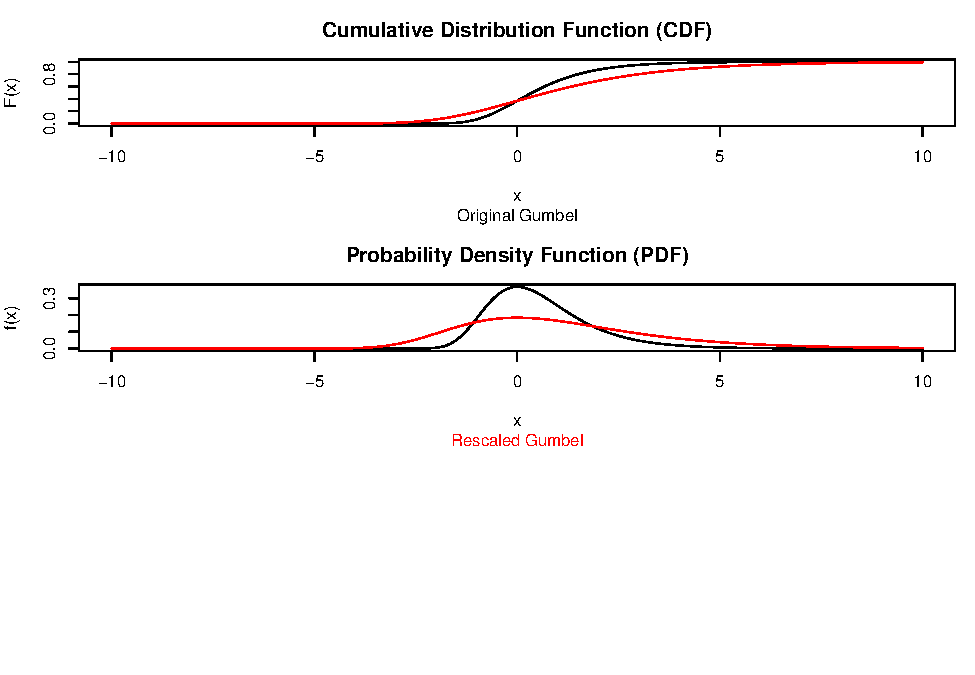
\includegraphics{extremales_files/figure-latex/gumbel_plots-1.pdf}
\caption{CDF and PDF for Gumbel distribution.}
\end{figure}

Si calculamos el valor esperado y el desvío estandard de estos valores
observados y tenemos una muestra lo suficientemente grande, podremos
comparar los resultados con los esperados de forma teórica.

\begin{Shaded}
\begin{Highlighting}[]
\CommentTok{\# Podemos simular 100 datos aleatorios de una distribución Gumbel}
\NormalTok{GumbelAleatorio}\OtherTok{\textless{}{-}}\FunctionTok{rgumbel}\NormalTok{(}\DecValTok{100}\NormalTok{)}
\FunctionTok{plot}\NormalTok{(}\FunctionTok{density}\NormalTok{(GumbelAleatorio))}
\end{Highlighting}
\end{Shaded}

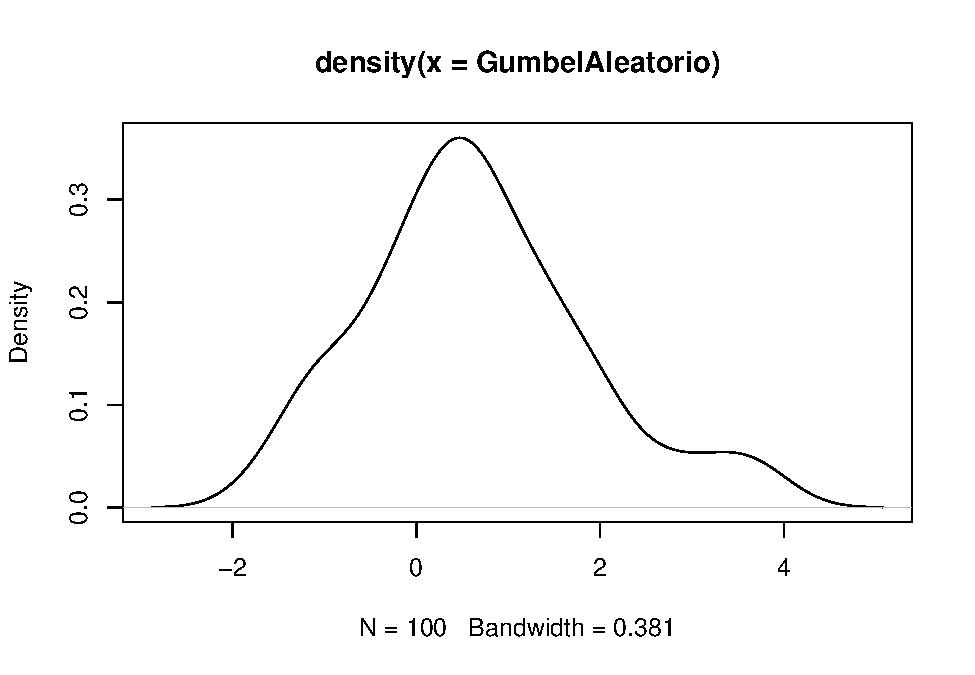
\includegraphics{extremales_files/figure-latex/unnamed-chunk-13-1.pdf}

\begin{Shaded}
\begin{Highlighting}[]
\SpecialCharTok{{-}}\FunctionTok{digamma}\NormalTok{(}\DecValTok{1}\NormalTok{) }\CommentTok{\# Constante de Euler{-}Mascheroni}
\end{Highlighting}
\end{Shaded}

\begin{verbatim}
## [1] 0.5772157
\end{verbatim}

\begin{Shaded}
\begin{Highlighting}[]
\FunctionTok{mean}\NormalTok{(}\FunctionTok{rgumbel}\NormalTok{(}\DecValTok{1000}\NormalTok{))}
\end{Highlighting}
\end{Shaded}

\begin{verbatim}
## [1] 0.5884223
\end{verbatim}

\begin{Shaded}
\begin{Highlighting}[]
\FunctionTok{sd}\NormalTok{(}\FunctionTok{rgumbel}\NormalTok{(}\DecValTok{1000}\NormalTok{))}
\end{Highlighting}
\end{Shaded}

\begin{verbatim}
## [1] 1.299118
\end{verbatim}

\hypertarget{distribuciuxf3n-de-weibull}{%
\subsubsection{Distribución de
Weibull}\label{distribuciuxf3n-de-weibull}}

Se dice que una variable tiene distribución de Weibull de orden
\(\alpha>0\) si su distribución es:

\[\Psi_{\alpha}(x)=\begin{cases}
exp{-(-x)^{\alpha}} & si\;x<0\\
1 & \text{en otro caso}
\end{cases}\] Recordemos que cuando tomamos los máximos de las variables
\(iid\) con un rango acotado, la distribución resultante por la cual se
puede aproximar es la de Weibull. En este caso, y en el resto del LAB,
exp() y e son la función exponencial.

Por una única vez, calculemos la distribución de forma ``manual'' en el
R para convencernos de la forma de la función de distribución de Weibull
(\(\Psi\)). Para eso generaremos un vector auxiliar de valores \(x\) y
la distribución (\(F(x)\)). En R la definición de la distribución es
sutilmente diferente a la que vimos en el teórico (definida para
positivos), pero totalmente convertible con dos cambios de signo. La
función que calcula la probabilidad de una distribución Weibull es
\textbf{pweibull()}. Pueden ver la definición de R utilizando
help(pweibull) o ?pweibull.En R podemos saber la forma y valores de esta
distribución con una función implementada en un paquete base \{stats\}.
La función es pweibull y lleva como argumentos un vector de cuantiles (
q ), un argumento de forma ( shape ) y otro de escala ( scale ).
Recordemos que la función plot utiliza 2 argumentos centrales ( x e y )
y podemos fijar los límites del gráfico ( xlim e ylim), el tipo de
gráfico ( type) y las etiquetas de los ejes X e Y ( xlab e ylab).

Primero generaremos un vector de numeros auxiliares equiespaciados y lo
nombraremos (``x\_aux''). Luego definiremos un orden (alpha=α ) de la
Weibull y graficaremos la función.

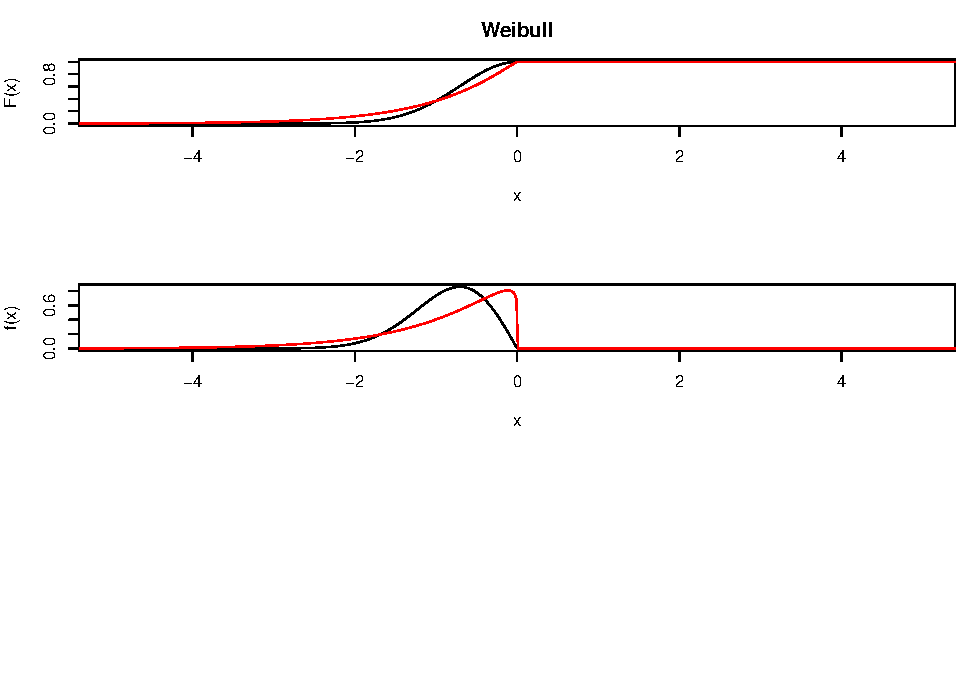
\includegraphics{extremales_files/figure-latex/unnamed-chunk-17-1.pdf}
Veamos ahora la forma de un par de distribuciones cambiando el parámetro
de orden (α ), que en la función pweibull de R se nombra como shape y
que define el orden de la distribución.

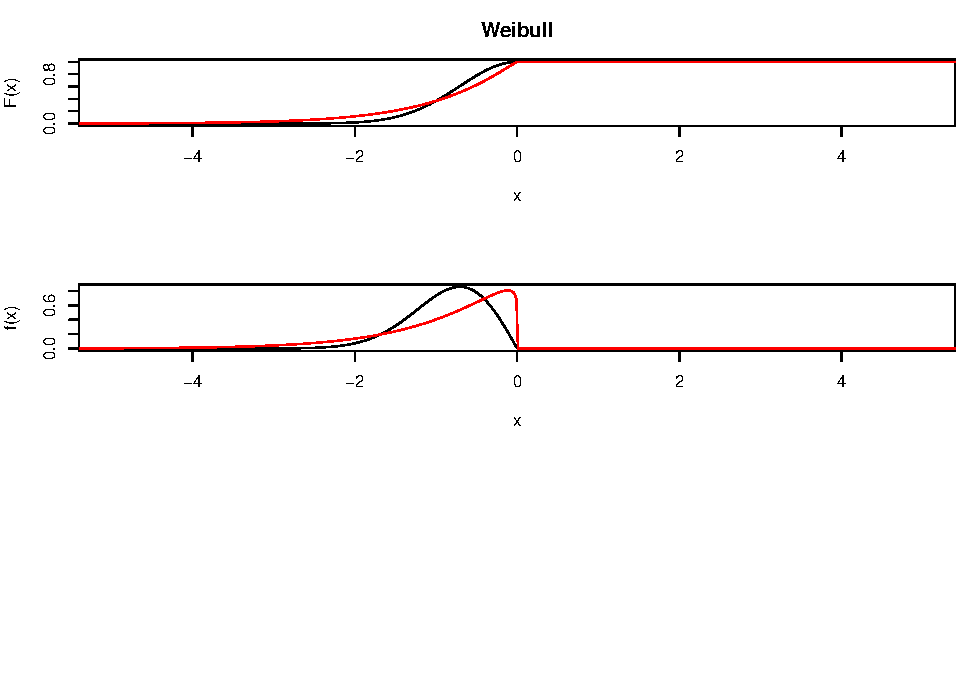
\includegraphics{extremales_files/figure-latex/unnamed-chunk-18-1.pdf}
En R podemos también generar numeros aleatórios (técnicamente
pseudo-aleatorios) de una distribución extremal. Estos simuladores de
números aleatórios son útiles para comparar contra distribuciones nulas,
generar modelos sintéticos para probar algorítmos, etc\ldots{} Para lxs
que venimos de la rama mas aplicada, muchas veces nos ayudan a entender
como funcionan los modelos y a verificar si nuestra intuición es
acertada respecto a la escala de ajuste de los parámetros entre otras
útiles. Generaremos 2 series de 1000 números aleatórios con la función
rweibull, que tiene como parámetro el número de datos que se necesitan y
la forma (shape) de la distribución. Luego haremos un grafico con la
densidad empírica (esto es similar a un histograma) de estos vectores.

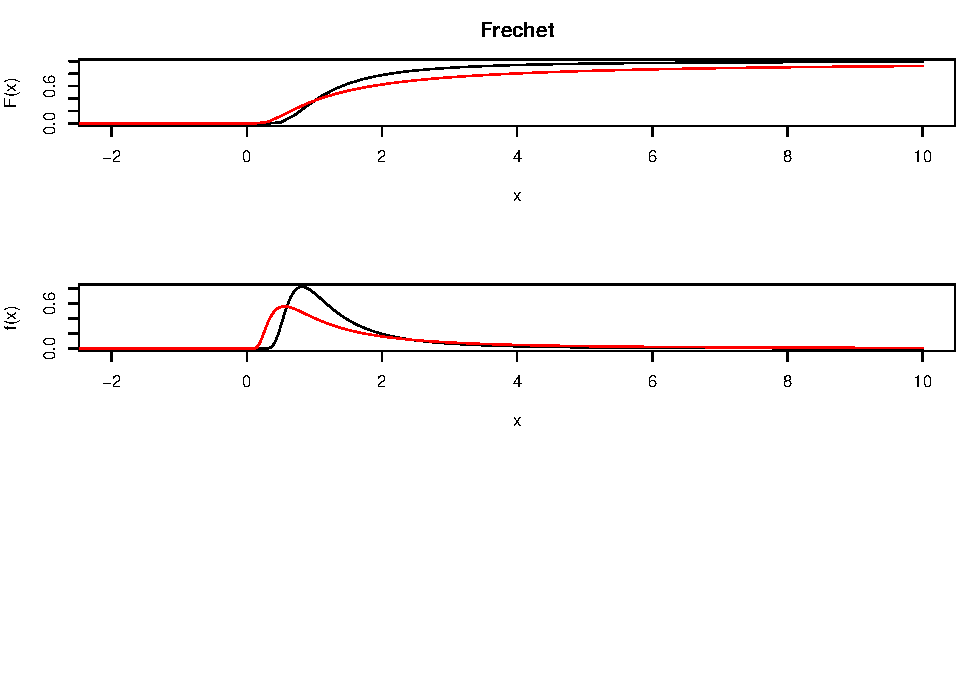
\includegraphics{extremales_files/figure-latex/unnamed-chunk-19-1.pdf}

\hypertarget{distribuciuxf3n-de-fruxe9chet}{%
\subsubsection{Distribución de
Fréchet}\label{distribuciuxf3n-de-fruxe9chet}}

Se dice que una variable tiene distribución de Fréchet de orden
\(\alpha>0\) si su distribución es:

\[
\Phi_{\alpha}(x)=\begin{cases}
exp\{-x^{-\alpha}\} & si\;x>0\\
0 & \text{en otro caso}
\end{cases}
\]

Esta tercera clase de variables incluyen a las distribuciones no
acotadas, pero de colas pesadas. Es decir que tienen una probabilidad
alta de presentar valores alejados de la media o la mediana (ej. la
Cauchy). En estos casos, la distribución de sus máximos es la Frechet.
Grafiquemos esta distribución para dos valores diferentes de \(\alpha\).

\begin{Shaded}
\begin{Highlighting}[]
\NormalTok{x\_aux}\OtherTok{\textless{}{-}} \FunctionTok{seq}\NormalTok{(}\SpecialCharTok{{-}}\DecValTok{10}\NormalTok{,}\DecValTok{10}\NormalTok{, }\AttributeTok{length=}\DecValTok{1000}\NormalTok{)}

\FunctionTok{par}\NormalTok{(}\AttributeTok{mfrow=}\FunctionTok{c}\NormalTok{(}\DecValTok{3}\NormalTok{,}\DecValTok{1}\NormalTok{), }\AttributeTok{mar=}\FunctionTok{c}\NormalTok{(}\DecValTok{5}\NormalTok{,}\DecValTok{4}\NormalTok{,}\DecValTok{3}\NormalTok{,}\DecValTok{1}\NormalTok{))}
\FunctionTok{plot}\NormalTok{(}\FunctionTok{seq}\NormalTok{(}\SpecialCharTok{{-}}\DecValTok{10}\NormalTok{,}\DecValTok{10}\NormalTok{,}\AttributeTok{length=}\DecValTok{100}\NormalTok{), }\FunctionTok{pfrechet}\NormalTok{(}\AttributeTok{q=}\FunctionTok{seq}\NormalTok{(}\SpecialCharTok{{-}}\DecValTok{10}\NormalTok{,}\DecValTok{10}\NormalTok{,}\AttributeTok{length=}\DecValTok{100}\NormalTok{), }\AttributeTok{shape=}\DecValTok{2}\NormalTok{, }\AttributeTok{scale=}\DecValTok{1}\NormalTok{) ,}\AttributeTok{xlim=}\FunctionTok{c}\NormalTok{(}\SpecialCharTok{{-}}\DecValTok{2}\NormalTok{,}\DecValTok{10}\NormalTok{), }\AttributeTok{type=}\StringTok{"l"}\NormalTok{, }\AttributeTok{ylab=}\StringTok{"F(x)"}\NormalTok{, }\AttributeTok{xlab=}\StringTok{"x"}\NormalTok{, }\AttributeTok{main=}\StringTok{"Frechet"}\NormalTok{)}
\FunctionTok{lines}\NormalTok{(}\FunctionTok{seq}\NormalTok{(}\SpecialCharTok{{-}}\DecValTok{10}\NormalTok{,}\DecValTok{10}\NormalTok{,}\AttributeTok{length=}\DecValTok{100}\NormalTok{), }\FunctionTok{pfrechet}\NormalTok{(}\AttributeTok{q=}\FunctionTok{seq}\NormalTok{(}\SpecialCharTok{{-}}\DecValTok{10}\NormalTok{,}\DecValTok{10}\NormalTok{,}\AttributeTok{length=}\DecValTok{100}\NormalTok{), }\AttributeTok{shape=}\FloatTok{1.1}\NormalTok{, }\AttributeTok{scale=}\DecValTok{1}\NormalTok{),}\AttributeTok{col=} \StringTok{"red"}\NormalTok{)}

\FunctionTok{plot}\NormalTok{(x\_aux, }\FunctionTok{dfrechet}\NormalTok{(}\AttributeTok{x=}\NormalTok{x\_aux, }\AttributeTok{shape=}\DecValTok{2}\NormalTok{, }\AttributeTok{scale=}\DecValTok{1}\NormalTok{, }\AttributeTok{log =} \ConstantTok{FALSE}\NormalTok{) ,}\AttributeTok{xlim=}\FunctionTok{c}\NormalTok{(}\SpecialCharTok{{-}}\DecValTok{2}\NormalTok{,}\DecValTok{10}\NormalTok{), }\AttributeTok{type=}\StringTok{"l"}\NormalTok{, }\AttributeTok{ylab=}\StringTok{"f(x)"}\NormalTok{, }\AttributeTok{xlab=}\StringTok{"x"}\NormalTok{)}
\FunctionTok{lines}\NormalTok{(x\_aux, }\FunctionTok{dfrechet}\NormalTok{(}\AttributeTok{x=}\NormalTok{x\_aux, }\AttributeTok{shape=}\FloatTok{1.1}\NormalTok{, }\AttributeTok{scale=}\DecValTok{1}\NormalTok{, }\AttributeTok{log =} \ConstantTok{FALSE}\NormalTok{), }\AttributeTok{col=}\StringTok{"red"}\NormalTok{)}
\end{Highlighting}
\end{Shaded}

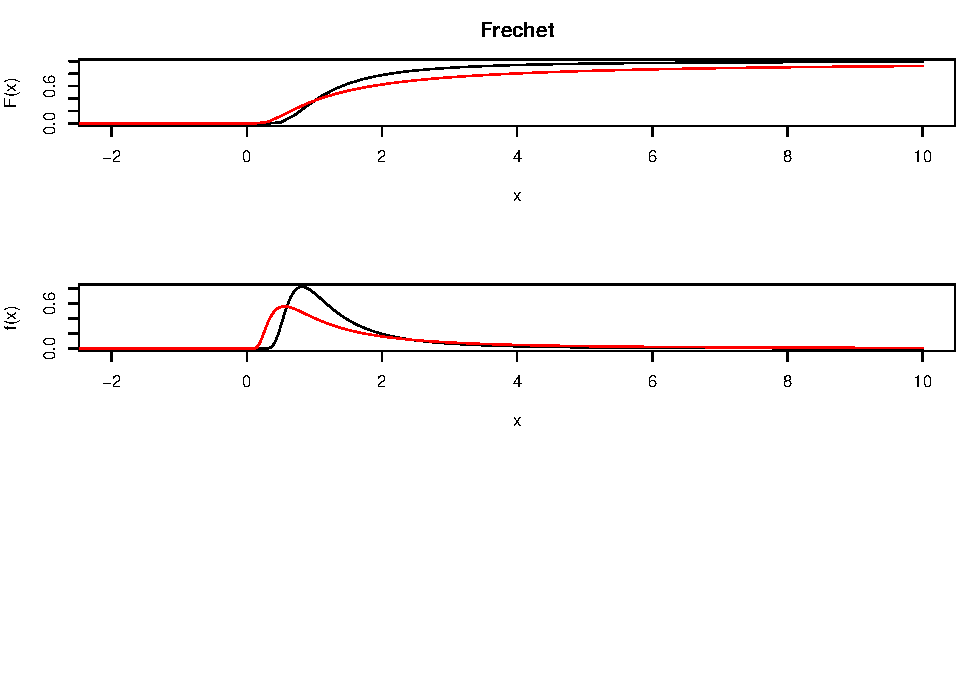
\includegraphics{extremales_files/figure-latex/unnamed-chunk-20-1.pdf}

.

\newpage

\hypertarget{teorema-1-relaciones-entre-las-versiones-standard-de-las-distribuciones-extremales}{%
\paragraph{Teorema 1: Relaciones entre las versiones standard de las
distribuciones
extremales}\label{teorema-1-relaciones-entre-las-versiones-standard-de-las-distribuciones-extremales}}

\(X\) tiene distribución \(\Phi_{\alpha}(x)\) si y sólo si \((-1/X)\)
tiene distribución \(\Psi_{\alpha}(x)\) si y sólo si \(log(X^{\alpha})\)
tiene distribución \(\Lambda\).

\hypertarget{teorema-2-algunos-datos-de-las-distribuciones-extremales}{%
\paragraph{Teorema 2: Algunos datos de las distribuciones
extremales}\label{teorema-2-algunos-datos-de-las-distribuciones-extremales}}

\hypertarget{parte-1}{%
\paragraph{Parte 1}\label{parte-1}}

Si \(X\) tiene distribución \(\Lambda^{(\mu,\beta)}\) entonces tiene:

\begin{itemize}
  \item[a)] Valor esperado: $E(X) = \mu + \beta\gamma$, donde $\gamma$ es la constante de Euler-Mascheroni, cuyo valor aproximado es $0.5772156649$.
  \item[b)] Moda: $\mu$
  \item[c)] Mediana: $\mu - \beta \log(\log 2) \approx \mu - 0.36651 \beta$.
  \item[d)] Desviación estándar: $\beta \pi \sqrt{6} \approx 1.2825 \beta$.
  \item[e)] Si $X^+ = \max(X,0)$, entonces $E(X+k)$ es finito para todo valor de $k$ natural.
  \item[f)] Para simular computacionalmente $X$, se puede tomar $U$ uniforme en $(0,1)$ y hacer $X = \mu - \beta \log(-\log U)$.
\end{itemize}

\hypertarget{parte-2}{%
\subsubsection{Parte 2}\label{parte-2}}

Si \(X\) tiene distribución \(\Psi_{\alpha}^{(\mu,\beta)}\) entonces
tiene:

\begin{itemize}
  \item[a)] Valor esperado: $E(X) = \mu + \beta\Gamma(1+1/\alpha)$.
  \item[b)] Moda: $\mu$ si $\alpha\leq 1$ y $\mu-\beta\{(\alpha-1)/\alpha\}^{(1/\alpha)}$ si $\alpha>1$.
  \item[c)] Mediana: $\mu - \beta \log(2)^{(1/\alpha)}$.
  \item[d)] Desviación estándar: $\beta\{\Gamma(1+2/\alpha)-\Gamma(1+1/\alpha)^2\}^{1/2}$.
\end{itemize}

\hypertarget{parte-2-1}{%
\subsubsection{Parte 2}\label{parte-2-1}}

Si \(X\) tiene una distribución \(\Phi_{\alpha}^{(\mu, \beta)}\)
entonces se tiene:

\begin{itemize}
  \item[a)] Valor esperado: $E(X) = \mu + \beta\Gamma(1-1/\alpha)$ si $\alpha > 1$, $\infty$ en caso contrario.
  \item[b)] Moda: $\mu + \beta\Gamma(1-1/\alpha)$ si $\alpha>1$.
  \item[c)] Mediana: $\mu + \beta \log(2)^{(-1/\alpha)}$.
  \item[d)] Desviación estándar: $\beta|\Gamma(1-2/\alpha)-\Gamma(1-1/\alpha)^2|$ si $\alpha>2$, $\infty$ si $1<\alpha \leq 2$.
\end{itemize}

\newpage

\hypertarget{teorema-3-fischer-tippet-gnedenko-ftg}{%
\paragraph{Teorema 3: Fischer-Tippet-Gnedenko
(FTG)}\label{teorema-3-fischer-tippet-gnedenko-ftg}}

Si \(X_1,...,X_n\quad iid\) con distribución \(F\) ``continua'',
llamamos \(F_n^*\) a la distribución de \(max(X_1,...,X_n)\) y \(n\) es
grande, entonces existen \(\mu\) real y \(\beta>0\) tales que alguna de
las siguientes tres afirmaciones es correcta:

\begin{itemize}
  \item[1)] $F_n^*$ se puede apromixar por la distribución de $\mu+\beta Y$ con $Y$ variable con distribución $\Lambda$.
  \item[2)] Existe $\alpha>0$ tal que $F_n^*$ se puede aproximar por la distribución de $\mu+\beta Y$ con $Y$ variable con distribución $\Phi_{\alpha}$. 
  \item[3)] Existe $\alpha>0$ tal que $F_n^*$ se puede aproximar por la distribución de $\mu+\beta Y$ con $Y$ variable con distribución $\Phi_{\alpha}$.
\end{itemize}

Lo anterior equivale a decir que la distribución del máximo de datos
\textit{continuos} e \(iid\), si \(n\) es grande, puede aproximarse por
una Gumbel, una Fréchet o una Weibull. Una aproximación será válida
dependiendo de la distribución de \(F\). En este sentido, cuando \(F\)
sea normal entonces \(F_n^*\) se puede aproximar como una Gumbel. Cuando
\(F\) sea uniforme, se puede aproximar \(F_n^*\) como una Weibull y
cuando \(F\) sea Cauchy entonces \(F_n^*\) se puede aproximar por una
Fréchet.

Más precisamente, cuál de las tres aproximaciones es la aplicable
depende de la cola de \(F\) (los valores de \(F(t)\) para valores
grandes de \(t\)). En concreto, Weibull aparece cuando \(F\) es la
distribución de una variable acotada por arriba (como la Uniforme),
Gumbel para distribuciones de variables no acotadas por arriba pero con
colas muy livianas (caso Exponencial y Normal) y Fréchet para colas
pesadas (caso
Cauchy)\footnote{Si bien  la hipótesis de continuidad de $F$ no es esencial, si $F$ tiene
la distribución Binomial o Poisson, por ejemplo, no se puede aplicar ninguna de las tres aproximaciones anteriores.}.

Como consecuencia del \(FTG\) cuando se tengan datos máximos, las
distribuciones maximales podrían ser candidatas de uno de los ajustes si

\begin{itemize}
\item la cantidad de registros es lo suficientemente grande
\item los registros son $iid$ aunque con versiones más generales del $FTG$ este supuesto puede no cumplirse
\end{itemize}

Como la mayoría de tests de ajustes suponen datos \(iid\), se van a
realizar dos tests de
aleatoriedad\footnote{En inglés se expresa como \textit{randomness}} a
los datos:

\begin{itemize}
\item  Runs up and down 
\item  Spearman correlation of ranks 
\end{itemize}

Se emplea la prueba de ajuste \(\chi^2\) que requiere seleccionar una
partición más o menos arbitraria de la recta real de intervalos siendo
importante que en cada intervalo haya una cantidad lo suficientemente
importante de datos de la muestra. En este sentido, se pueden tomar como
extremos de los intervalos los quintiles empíricos de la muestra. Cabe
mencionar que este test requiere estimar parámetros por el método de
Máxia Verosimilitud Categórica.

Cabe mencionar que para este estudio la distribución de la variable a
incorporar en este estudio no tiene que ser degenerada, es decir
\(H(t)=0\) ó \(H(t)=1\).

\newpage

\hypertarget{definiciuxf3n-2-distribuciuxf3n-extremal-asintuxf3tica}{%
\subsection{Definición 2: Distribución extremal
asintótica}\label{definiciuxf3n-2-distribuciuxf3n-extremal-asintuxf3tica}}

Si \(X_1,...,X_n\) es \(iid\) con distribución \(F\) diremos que \(H\)
no-degenerada es la Distribución Extremal Asintótica (DEA) de
\(F\)\footnote{Lo que equivale a decir que $F$ tiene $DEA\;H$.}, si
existen dos sucesiones de números reales, \(d_n\) y \(c_n>0\), tales que
la distribución de

\begin{equation}
\frac{max(X_1,...,X_n)- d_n}{c_n}\label{eq:max}
\end{equation}

tiende a \(H\) cuando \(n\) tiende a infinito.

\hypertarget{definiciuxf3n-3-supremo-esencial-de-una-variable-aleatoria-o-distribuciuxf3n}{%
\subsection{Definición 3: Supremo esencial de una variable aleatoria o
distribución}\label{definiciuxf3n-3-supremo-esencial-de-una-variable-aleatoria-o-distribuciuxf3n}}

Si \(X\) tiene distribución \(F\), se llama supremo esencial de \(X\),
denotado como \(M_X\) o, indistintamente, supremo esencial de \(F\),
denotado \(MF\) a

\begin{equation}
M_X=M_F= sup\{t / F(t)<1\}\label{eq:Mx}
\end{equation}

Observación:

\begin{itemize}
\item Si $F$ es $U(a,b)$, $M_F=b$
\item Si $F$ es $Bin(m,p)$, $M_F=m$
\item Si $F$ es Normal, Exponencial, Cauchy o Poisson, $M_F$ es infinito.
\end{itemize}

\hypertarget{teorema-4}{%
\paragraph{Teorema 4}\label{teorema-4}}

Si \(X_1,...,X_n\) es \(iid\) con distribución \(F\) cualquiera,
entonces, para \(n\) tendiendo a infinito,

\begin{equation}
X^*_n=M_F= max(X_1,...,X_n)\;tiende\;a\;M_F\label{eq:Xast}
\end{equation}

Observación:

El resultado anterior vale incluso si \(M_F\) es infinito, pero si
\(M_F\) es finito, como \(X^*n - M_F\) tiende a cero, por analogía con
el Teorema Central del Límite para promedios, buscaríamos una sucesión
\(c_n>0\) y que tienda a cero de modo tal que \((X^*n- M_F )/ c_n\)
tienda a una distribución no-degenerada y de allí surge buscar la DEA.

\hypertarget{teorema-5}{%
\paragraph{Teorema 5}\label{teorema-5}}

Si \(F\) es una distribución con \(M_F\) finito, y para \(X\) con
distribución \(F\) se cumple que

\[
P(X=M_F)>0 
\]

entonces \(F\) NO admite DEA.

Observación:

Si \(F\) es \(Bin(m,p)\), \(M_F=m\). Si \(X\) tiene distribución \(F\),
entonces \(P( X=M_F)= P( X=m)= p_m>0\), asi que la distribucion
\(Bin(m,p)\) NO admite DEA, no se puede aproximar la distribución del
máximo de una muestra \(iid\) de variables \(Bin(m,p)\).

El Teorema anterior es un caso particular del próximo.

\hypertarget{teorema-6}{%
\paragraph{Teorema 6}\label{teorema-6}}

Si \(F\) es una distribución con \(M_F\) finito o infinito que admite
DEA, y \(X\) tiene distribución \(F\), entonces el límite cuando \(t\)
tiende a \(M_F\) por izquierda de \(P(X>t)/P(X \geq t)\) debe ser 1.

Observación:

\begin{itemize}
\item Si $F$ es una distribución de Poisson de parámetro $\lambda>0$, $M_F$ es infinito. 
\item Si $k$ es un natural, entonces:
\begin{eqnarray}
\frac{P(X>k)}{P(X\geq k)} &=& \frac{P(X \geq k+1)}{P(X\geq k)} \\ \nonumber
&=& 1-\frac{P(X=k)}{P(X \geq k)} \approx 1-\left(1- \frac{\lambda}{k}\right) 
\end{eqnarray}
que tiende a $0$ cuando $k$ tiende a infinito, por lo cual $F$ NO admite DEA, o sea que no se puede aproximar el máximo de una sucesión $iid$ de variables de Poisson.
\end{itemize}

Observación:

El Teorema 6 brinda una condición NECESARIA pero NO SUFICIENTE para DEA.
Un ejemplo de ello lo aportó Von Mises, mostrando que la distribución

\[F(x)= 1- e^{(-x-sen(x))}\] cumple con la condicion del Teorema 6 pero
no admite DEA.

\hypertarget{definiciuxf3n-4-distribuciuxf3n-max-estables}{%
\subsection{Definición 4: Distribución
max-estables}\label{definiciuxf3n-4-distribuciuxf3n-max-estables}}

Si dada una \(F\) distribución, \(X\) con distribución \(F\), \(k\)
natural arbitrario y \(X_1,...,X_k\) es \(iid\) con distribución \(F\),
existen reales \(a_k\), \(b_k\) tales que \(max(X_1,...,X_k)\) tiene la
misma distribución que \(a_k X+ b_k\), \(F\) se dice
\textit{max-estable}.

El Teorema FTG resulta de superponer los dos siguientes teoremas:

\hypertarget{teorema-7}{%
\paragraph{Teorema 7}\label{teorema-7}}

\begin{itemize}
  \item[a)] Si $F$ admite $DEA\;H$, entonces $H$ es max-estable.
  \item[b)] Si $H$ es max-estable, es la DEA de sí misma.
\end{itemize}

\hypertarget{teorema-8}{%
\paragraph{Teorema 8}\label{teorema-8}}

Una distribución es max-estable si y solo si es
extremal\footnote{O sea Gumbel, Weibull o Fréchet}. El Teorema 7 es
bastante intuitivo y análogo a los teoremas de Lévy sobre distribuciones
estables en aproximaciones asintóticas de las distribuciones de sumas.
Para el Teorema 8 haremos enseguida un ejercicio sencillo que nos
ayudará a hacerlo creíble. Luego precisaremos, para terminar con esta
parte, cómo son las distribuciones que tienen por DEA cada uno de los
tres tipos de distribuciones extremales. Para eso precisamos recordar
algunas definiciones, como la siguiente.

Obsrvación:

Si \(F\) y \(G\) son dos distribuciones, tienen colas equivalentes si
\(M_F=M_G\) y cuando \(t\) tiende a \(M_F\) por izquierda,
\((1-F(t))/(1-G(t))\) tiende a un valor \(c>0\). Recordando ahora cómo
se calcula la distribución del máximo de dos variables independientes,
es muy sencillo calcular la distribución del \(max\{X,Y\}\), cuando
\(X\) e \(Y\) son independientes y cada una de ellas es una distribución
extremal.

Se tiene el siguiente resultado:

\begin{longtable}[]{@{}
  >{\raggedright\arraybackslash}p{(\columnwidth - 4\tabcolsep) * \real{0.2500}}
  >{\raggedright\arraybackslash}p{(\columnwidth - 4\tabcolsep) * \real{0.2500}}
  >{\raggedright\arraybackslash}p{(\columnwidth - 4\tabcolsep) * \real{0.5000}}@{}}
\toprule\noalign{}
\begin{minipage}[b]{\linewidth}\raggedright
\(X\)
\end{minipage} & \begin{minipage}[b]{\linewidth}\raggedright
\(Y\)
\end{minipage} & \begin{minipage}[b]{\linewidth}\raggedright
\(max(X,Y)\)
\end{minipage} \\
\midrule\noalign{}
\endhead
\bottomrule\noalign{}
\endlastfoot
\textcolor{red}{Weibull} & \textcolor{red}{Weibull} &
\textcolor{red}{Weibull} \\
\textcolor[rgb]{0.0,0.5,0.0}{Weibull} &
\textcolor[rgb]{0.0,0.5,0.0}{Gumbel} &
\textcolor[rgb]{0.0,0.5,0.0}{Cola equivalente Gumbel} \\
\textcolor{blue}{Weibull} & \textcolor{blue}{Fréchet} &
\textcolor{blue}{Fréchet} \\
\textcolor[rgb]{0.0,0.5,0.0}{Gumbel} &
\textcolor[rgb]{0.0,0.5,0.0}{Weibull} &
\textcolor[rgb]{0.0,0.5,0.0}{Cola equivalente Gumbel} \\
\textcolor{red}{Gumbel} & \textcolor{red}{Gumbel} &
\textcolor{red}{Gumbel} \\
\textcolor{blue}{Gumbel} & \textcolor{blue}{Fréchet} &
\textcolor{blue}{Cola equivalente Fréchet} \\
\textcolor{blue}{Fréchet} & \textcolor{blue}{Weibull} &
\textcolor{blue}{Fréchet} \\
\textcolor{blue}{Fréchet} & \textcolor{blue}{Gumbel} &
\textcolor{blue}{Cola equivalente Fréchet} \\
\textcolor{red}{Fréchet} & \textcolor{red}{Fréchet} &
\textcolor{red}{Fréchet} \\
\end{longtable}

\textcolor{red}{\rule{1em}{1em} Las extremales son max-estables: tomar máximos de dos del mismo tipo queda en el mismo tipo.}

\textcolor[rgb]{0.0,0.5,0.0}{\rule{1em}{1em} Gumbel es más pesada que Weibull. En la cola, que es lo que cuenta para máximos, prima Gumbel.}

\textcolor{blue}{\rule{1em}{1em} Fréchet es más pesada que Gumbel y mucho más pesada que Weibull.}
\vspace{1cm}

Además, de la tabla se deduce que

\hypertarget{teorema-9}{%
\paragraph{Teorema 9}\label{teorema-9}}

Si \(X_1,...,X_n\) independientes y cada \(X_i\) tiene uno de los tres
tipos de distribución extremal, entonces la distribución del
\(max(X_1,...,X_n)\) es:

\begin{itemize}
\item[a)] Cola equivalente a Fréchet, si alguna de las variables es Fréchet y alguna otra es Gumbel.
\item[b)]  Fréchet, si alguna es Fréchet y ninguna es Gumbel.
\item[c)]  Cola equivalente Gumbel ninguna es Fréchet pero algunas son Gumbel y otras Weibull.
\item[d)] Gumbel si todas son Gumbel.
\item[e)]  Weibull si todas son Weibull.
\end{itemize}

Observación:

Si \(F\) es una distribución, se dice que tiene
\textit{cola de variación regular de orden} \(-\alpha\), para
\(\alpha \geq 0\), si para todo \(t>0\), \((1-F(tx))/(1-F(x))\) tiende a
\(t^{-\alpha}\) si \(x \rightarrow \infty\). Para abreviar se dirá que
\(F\) es \(R_{-\alpha}\). Por ejemplo, para \(\alpha=3\), un caso de una
tal \(F\) es \(F(u)=1- 1/u^3\).

Por otra parte se dice que \(L\) es una
\textit{función de variación lenta} si, para todo \(t>0\),
\(L(tx)/L(x)\) tiende a 1 cuando \(x \rightarrow \infty\). Por ejemplo,
\(L(u)=log(u)\).

\newpage

\hypertarget{definiciuxf3n-4-dominio-de-atracciuxf3n-maximal}{%
\subsection{Definición 4: Dominio de atracción
maximal}\label{definiciuxf3n-4-dominio-de-atracciuxf3n-maximal}}

Si \(H\) es una distribución extremal (Gumbel, Weibull o Fréchet) su
Dominio de Atracción Maximal (\(DAM(H)\)) está constituído por todas las
distribuciones \(F\) que tienen \(DEA\;H\).

\hypertarget{teorema-9-dam-de-la-fruxe9chet}{%
\paragraph{Teorema 9: DAM de la
Fréchet}\label{teorema-9-dam-de-la-fruxe9chet}}

\(F\) pertenece a la DAM de \(\Phi_{\alpha}\) si y sólo si
\(1-F(x)=x-\alpha L(x)\) para alguna \(L\) de variación lenta, lo cual
es equivalente a decir que \(F\) es \(R_{-\alpha}\).

\hypertarget{corolario-1-dam-de-la-fruxe9chet}{%
\paragraph{Corolario 1: DAM de la
Fréchet}\label{corolario-1-dam-de-la-fruxe9chet}}

Si \(F\) es una distribución con densidad \(f\) que cumple que
\(xf(x)/(1-F(x))\) tiende a \(\alpha\) cuando \(x \rightarrow \infty\)
se dice que \(F\) cumple la Condición de Von Mises I. En tal caso, \(F\)
pertenece a la DAM de \(\Phi_{\alpha}\) y mas aún, la DAM de
\(\Phi_{\alpha}\) son todas las distribuciones que tienen cola
equivalente a alguna distribución que cumpla la Condición de Von Mises
I. Del DAM Fréchet y Teorema 1, surge lo siguiente.

\hypertarget{teorema-10-dam-de-la-weibull}{%
\paragraph{Teorema 10: DAM de la
Weibull}\label{teorema-10-dam-de-la-weibull}}

\begin{itemize}
\item [a)] $F$ pertenece a la DAM de $\Psi_{\alpha}$ si y solo si $M_F$ es finito y además $$1-F(M_F -1/x)=x^{-\alpha} L(x)$$ para alguna
$L$ de variación lenta, es decir que pertenece a $R_{-\alpha}$. Observar que con el cambio de variable $u=M_F -1/x$,
resulta que $1-F(u)=(^{-}MF -u)^{\alpha} L(1/(M_F -u))$ para alguna $L$ de variación lenta, para $u< M_F$. Además puede tomarse $d_n= M_F$ y $c_n= n-\alpha$.
\item [b)] Si $F$ distribución con densidad $f$ positiva en $(a,M_F)$ para algun $a< M_F$ y $(M_F -x)f(x)/(1-F(x))$ tiende a $\alpha$ cuando $x\rightarrow M_F$, se dice que $F$ cumple la Condición de Von Mises II. En tal caso $F$ pertenece a la DAM de $\Psi_{\alpha}$ y mas aún, la DAM de $\Psi_{\alpha}$ son todas las distribuciones que tienen cola equivalente a alguna distribución que cumpla la Condición de Von Mises II.
\end{itemize}

\hypertarget{teorema-11-dam-de-la-gumbel}{%
\paragraph{Teorema 11: DAM de la
Gumbel}\label{teorema-11-dam-de-la-gumbel}}

Una distribución \(F\) se dice una Función de Von Mises con función
auxiliar \(h\) si existe \(a < M_F\) (\(M_F\) puede ser finito o
infinito) tal que para algún \(c>0\) se tiene

\[
1-F(x)= c\;exp^{{- \int_a^X \frac{1}{h(t)} dt}},
\]

con \(h\) positiva, con densidad \(h^\prime\) y \(h^\prime(x)\)
tendiendo a \(0\) para \(x\rightarrow M_F\) Se tiene entonces que la
\(DAM\) de \(\Lambda\) son todas las distribuciones que tienen cola
equivalente a alguna distribución que sea una Función de Von Mises.
Básicamente, se trata de colas más livianas que cualquier expresión del
tipo \(1/x^k\), más aún, con decaimiento \textit{del tipo exponencial},
en el sentido preciso siguiente: si como en el Teorema 11

\(1-F(x)= c\;exp^{{- \int_a^X \frac{1}{h(t)} dt}}\), entonces se tiene
\(1-F(x)= c\;exp^{-(x-a)/h(x)}\), donde la función auxiliar \(h\) es
no-decreciente y con asíntota horizontal.

Además, \(d_n\) y \(c_n\) suelen involucrar expresiones logarítmicas.
Más concretamente, \(dn = F^{-1}(1-1/n)\), \(c_n = h(d_n)\), donde
\(F^{-1}\) es la inversa generalizada (o función cuantil), definida por
\(F^{-1}(p)= inf\{t / F(t)\geq p\}\), para \(0<p<1\).

\hypertarget{corolario-2}{%
\subsection{Corolario 2 :}\label{corolario-2}}

Si \(F\) pertenece al \(DAM\) Gumbel, \(M_F\) es infinito, y se
considera \(X\) con distribucion \(F\), entonces \(E(X+k)\) es finito
para todo \(k\) natural. Los resultados antes vistos nos permiten
reconocer que distribuciones tienen \(DEA\) y si la tienen, cual es.
Cierran el tema. Adicionalmente, permiten ver con mucha precision que el
quid de esta teoría es el comportamiento de las colas de las
distribuciones, que Fréchet corresponde a las colas más pesadas, luego
la Gumbel y finalmente Weibull. Para terminar el capítulo presentaremos
la distribución de valores extremos
generalizada\footnote{GEV, por sus siglas en inglés.}, que es una forma
de compactar en una unica fórmula las tres distribuciones extremales,
debida a Jenkinson-Von Mises.

\hypertarget{definiciuxf3n-5-gev}{%
\subsection{Definición 5: GEV}\label{definiciuxf3n-5-gev}}

Se define a la distribución de valores extremos generalizada
\((GEV)\)\footnote{Por sus siglas en inglés relativas a Generalized Extreme Values.}
de posición \(\mu\), escala \(\beta\) e índice \(\xi\) con

\[
G(\mu,\beta,\xi) =
\begin{cases}
    e^{-(1+ \xi(t-\mu)/ \beta)(-1/ \xi)} & \text{si  } \xi \neq 0, \forall\;t\;\text{donde } 1+ \xi(t-\mu)/ \beta) >0 \\
    e^{-e^{(-(t-\mu)/ \beta)}} & \text{si  } \xi =0,\; \forall \;t \\
\end{cases}
\] \vspace{0.5cm}

En los casos en que \(\xi\) tome los siguientes valores, se tiene

\begin{align*}
 \xi=0,  & \text{ corresponde a Gumbel,} \\
 \xi< 0, &\text{ corresponde a Weibull y } \alpha=-1/ \xi \\
 \xi>0, &\text{ corresponde Fréchet y }  \alpha=1/ \xi
\end{align*}

En \(R\) existen rutinas para estimar \(\xi\) con intervalos de
confianza( por máxima verosimilitud, etc.) lo cual da formas de testear
si una extremal es Gumbel, Weibull o Fréchet.

Observación:

En algunas situaciones datos extremales pueden ajustarse a más de un
modelo. Por ejemplo, puede ocurrir que tanto ajusten los datos una
Gumbel como una Weibull. Frente a estas situaciones, no hay una receta
única de cómo proceder sino que quien está modelando debe tener claro si
corresponde volcarse hacia cálculos más pesimistas (que dan mayor
probabilidad a eventos extremos muy severos) o más optimistas.

Usualmente la opción pesimista implica privilegiar la seguridad y la
optimista la economía de recursos, pero insistimos en que la reflexión
ante cada caso es indispensable. Un poquito más adelante veremos, al
comparar un modelo Gumbel con un modelo Fréchet, que las diferencias
pueden ser sumamente drásticas.

Observación:

Antes de seguir adelante, demos la respuesta a la parte \(a)\) del
Ejercicio 5. Es un ejercicio de Cálculo Diferencial sencillo mostrar que
la cola de un \(N(0,1)\), es decir \(Q(t)=P(X>t)\), donde \(X\) tiene
distribución \(N(0,1)\), es equivalente, para \(t\) tendiendo a
infinito, a la función \(\phi(t)/t\), donde \(\phi\) representa la
densidad normal típica (campana de Gauss). Basándose en esto, si se
considera ahora una variable log-normal \(Y\), tal que \(log(Y)\) es una
\(N(0,1)\), puede probarse que su cola \(R(t)=P(Y>t)\), es equivalente,
para \(t\) tendiendo a infinito, a la función \(\phi(log(t))/log(t)\).
Con un poco más de Cálculo, esta última función puede escribirse para
\(a>e\) (por ejemplo \(a=3\)), como

\begin{equation}
c\times e^{-\int_{a}^{t}1/h(s)\; ds} \quad \text{para }\: t>a
\end{equation}

donde \(c\) se expresa en función de \(a\) y
\(h(s)=\frac{s\; log(s)}{(log(s))^2+1}\) la cual cumple las hipótesis
del Teorema 11.

Se concluye entonces que la log-normal está en el \(DAM\) Gumbel, o lo
que es lo mismo, que la log- normal admite \(DEA\) Gumbel.

Observación: Tiempos y Valores de Retorno

En Ingeniería y Ciencias Ambientales, suele pensarse los eventos
extremos (por ejemplo: observación por encima de cierto valor muy alto),
en términos de tiempos de retorno (tiempo que se espere para que ocurra
un evento). Bajo las hipótesis de datos \(iid\), el tiempo de retorno
\(T\) tiene una distribución \(Geo(p)\), con \(p = P(evento)\), por lo
cual el tiempo de retorno medio es \(E(T)=1/p\) y pueden hacerse
intervalos de confianza para \(E(T)\), en la medida que exista
información de \(P(evento)\), lo cual puede obtenerse a partir de este
capítulo o de los siguientes. Cabe observar que muchas veces se utiliza
la expresión Tiempo de Retorno (TR) para \(E(T)\).

Más precisamente, \(TR(u)\), el Tiempo de retorno del valor \(u\), es el
valor esperado (o la media) del tiempo que se debe esperar para que la
variable en estudio supere el valor \(u\), es decir que
\(TR(u) = 1/P(X>u)\), si \(X\) es la variable en estudio.

Por otro la lado, en una mirada inversa, el Valor de Retorno a tiempo
\(t\), \(VR(t)\) es el valor de \(u\) para el cual \(TR(u)=t\), es decir
que \(TR(VR(t))=t\) (y también \(VR(TR(u))=u\), es decir que \(TR\) y
\(VR\) son, como funciones, inversas una de la otra).

Para \textit{bajar un poco a tierra} estos conceptos, vamos a
calcularlos y compararlos cuando la variable \(X\) es Gumbel y cuando
(con los mismos valores de posición \(\mu\) y escala \(\beta>0\)).

Comencemos por la Gumbel, recordemos que \(X\) tiene distribución
\(\Lambda( \mu,\beta)\) si \(X= \mu+\beta Y\) , donde \(Y\) tiene
distribución \(\Lambda\).

Dado entonces un valor \(\mu>0\) , otro valor \(t>0^*\) resulta que

\begin{itemize}
\item $P(X>u)=1-e^{-e{(u-\mu)/ β }}$
\item $TR(u)=1/P(X>u)$
\item $VR(t)= \mu-\beta\: log\{log\{t/(t-1)\}\}$
\end{itemize}

(ECUACIONES
G)\footnote{Cabe observar que si se supone que las observaciones son diarias (o enteras en la unidad que corresponda), los tiempos de retorno TR se redondean a enteros y los valores de $t$ en la última ecuación se toman enteros.}

Sigamos ahora por la Fréchet, recordemos que \(X\) tiene distribución
\(\Phi_{\alpha}^{( \mu,\beta)}\) si \(X= \mu+\beta Y\), donde \(Y\)
tiene distribución \(\Phi_{\alpha}\).

Dado entonces un valor \(u>0\), otro valor \(t\) entero, resulta que

\begin{itemize}
\item $P(X>u)=1-e^{ -\left \{( u- \mu)/\beta\right \}^{-\alpha}}$,
\item $TR(u)=\frac{1}{P(X>u)}$,
\item $VR(t)= \mu+ \beta\left \{log\left \{ \frac{t}{(t-1)}\right \}\right \}-\frac{1}{\alpha}$
\end{itemize}

(ECUACIONES F)

Para visualizar claramente estos resultados, tabularemos y graficaremos
los mismos usando en ambos casos:

\begin{itemize}
\item $\mu=15$
\item $\beta=10$
\item $\alpha=2.5$
\item $\xi=0.4$ no muy distante del $\xi=0$ de la Gumbel
\end{itemize}

\begin{Shaded}
\begin{Highlighting}[]
\CommentTok{\# faltan datos, ya los pedí}
\end{Highlighting}
\end{Shaded}

Tanto las tablas como la gráfica muestran que el modelo Fréchet da
probabilidades mucho mayores a valores muy elevados (es más
``pesimista'', si los valores mayores representan mayores esfuerzos o
problemas).

Tratemos de ver ahora los TR para uno y otro modelo. Es claro que,
siguiendo la lógica anterior, es más ``pesimista'' el modelo que de
tiempos de retorno menores en valores elevados.

\begin{Shaded}
\begin{Highlighting}[]
\CommentTok{\#datos}
\end{Highlighting}
\end{Shaded}

Se observa muy claramente que el modelo Fréchet es mucho más
``pesimista''. Veamos ahora los VR. Será en este contexto más
``pesimista'' quien dé mayores VR.

Resulta evidente el mayor ``pesimismo''del modelo Fréchet. Finalmente,
para cerrar el punto, veamos que TR y VR son efectivamente inversas.

Por ejemplo, si tomamos el tiempo \(t=90\) días, vemos que en Gumbel su
\(VR\) es \(59,942\) muy ligeramente inferior a 60. En la tabla de TR,
vemos que para el valor 60, Gumbel da TR= 91, casi igual a t=90. Si con
este mismo \(t\) vamos al modelo Fréchet, vemos que su VR es 75,537 algo
superior a 74.

En la tabla de TR vemos que para el valor 75 Fréchet da TR= 89, casi
igual a t=90.

Es decir que, salvando las ligeras diferencias fruto de que las tablas
son discretas y hay redondeos, etc., hemos corroborado que para \(t\)
días, tenemos que TR \((VR(t))=t\). Si tomamos ahora el valor 70, vemos
que en Gumbel tiene TR=245, un poco por debajo de 270, cuyo
\(VR=70,966\). En Fréchet 70 tiene \(TR=71\), más abajo que 90, que
tiene \(VR= 75,357\) bastante cercano a 70. Haciendo la salvedad de lo
artesanal y aproximado de mirar una tabla y no calcular en continuo,
queda claro que para un valor u tenemos que \(VR(TR(u))=u\).

\newpage
\chapter{Un primer enfoque de datos no iid}

Vamos a ver que en la realidad frecuentemente los datos no son
\(i.i.d\), y que hay muy diversos tipos de datos no \(i.i.d\).

Recordemos que si los datos no son \(i.i.d\) es, o bien porque no son
independientes, o bien porque la distribución no es la misma para todos
los datos (o ambas cosas, obviamente).

\textbf{Aclaración 1:}

Dado que abordamos un curso de posgrado, y que en los cursos básicos se
abordan los tests que permiten contrastar la hipótesis iid (Spearman,
runs up and down, etc.) supondremos estas técnicas conocidas, pero
obviamente podemos analizarlas aparte con quien lo necesite. En R, por
ejemplo, se encuentran como \textbf{randtests}. Un escalón más arriba,
las Series de Tiempo, su análisis espectral, etc., es tema de otros
curso de segundo nivel de Estadística que ofrecemos, por lo cual no nos
detendremos mayormente, pero nuevamente, estamos a disposición de quien
lo requiera y en este curso al menos explicaremos brevemente los
aspectos medulares que usemos.

\textbf{Aclaración 2:}

En la teoría de series de tiempo, se suele expresar la expresión ``Ruido
Blanco'' para referirse a datos iid. Se caracterizan por tener espectro
constante. Hay por lo tanto tests basados en el Periodograma (estimación
de la medida espectral del proceso) que permiten testear si tenemos un
ruido blanco, o, más en general, qué tipo de estructura de dependencia
tienen los datos, permitiendo dilucidar entre alternativas que
presentaremos a continuación.

Continuando con una explicación ``llana'' del tema, si los datos no
necesariamente son independientes pero la estructura de distribuciones
es siempre la misma, se habla de datos estacionarios (o procesos
estacionarios).

Cuando los datos no son independientes pero la dependencia se va
atenuando a medida que se consideran datos más lejanos (para fijar
ideas, imaginemos que los datos corresponde a medidas en el tiempo, y
que datos muy viejos no influirían significativamente sobre el presente,
por ejemplo), se habla de datos débilmente dependientes.

El caso más sencillo de esta situación es la de datos m-dependientes
(donde m es un número), que corresponde a datos que si están a distancia
mayor a m, son independientes. Es el caso de los procesos \(MA(q)\) (
Moving Averages), que son Promedios Móviles de orden q de un ruido
blanco (\(m=q\) en este caso).

Algunos datos bioquímicos del agua de algunas playas uruguayas que se
miden diariamente suelen ser 7-dependientes, por ejemplo. Esto significa
que datos que fueron tomados con más de una semana de separación, son
independientes. En cambio, algunos datos de poblaciones o de
composici;on de suelos que se van registrando a lo largo de los años,
son débilmente dependientes, pero NO son m-dependientes para ningún m.
Es el caso, por ejemplo, de los llamados procesos \(AR(p)\)
(Autoregresivos de orden \(p\)) donde cada dato es una combinación
lineal de los p anteriores más un término aleatorio (``Ruido'') que es
un ruido blanco. Son Markovianos, es decir, con memoria infinita pero
donde todo el pasado es tan informativo como los últimos p datos (el
carácter Markoviano es mal presentado en algunos textos y cursos,
hablando confusamente de ``memoria corta'').

La Genética aporta excelentes ejemplos para distinguir lo Markoviano,
pues algunas pocas generaciones atrás alcanzan para calcular
probabilidades de muchas características de la descendencia, mientras
que la memoria no es corta sino infinita: cada característica resulta de
toda la fiogenética, así nos remontemos al origen de las especies. Para
simplificar al extremo y usando la imagen bíblica (con todo respeto a
todos los pensares), si Adán y Eva hubieran tenido otros genes, la
especie podría ser diferente!!

En la teoría clásica de series de tiempo, una estructura \(AR(p)\) a
partir de un ruido \(MA(q)\) en lugar de un ruido blanco, da lugar a los
procesos \(ARMA (p,q)\), que en general son débilmente dependientes y
aproximan bien a cualquier proceso estacionario débilmente dependiente,
lo cual es una de las razones de su popularidad. Lo opuesto a
dependencia débil es dependencia fuerte ( en inglés, long range
dependence). En algunos datos de telecomunicaciones que se registran en
escalas temporales muy finas, se han encontrado ejemplos de dependencia
fuerte.

Cuando los datos no son \(i.i.d.\) pero se vuelven \(i.i.d.\) al
restarle una función determinística, son bastante simples de manejar. Si
esta función es monótona, se habla de que los datos presentan tendencias
(trends). Si en cambio la función es periódica, se dice que los datos
presentan ciclos (seasonal effects). Se puede demostrar que si los datos
se vuelven iid al restar una función determinística cualquiera (lo cual
no siempre es el caso!), entonces se pueden modelar aproximadamente como

\[
\text{TENDENCIAS+CICLOS+ DATOS IID}
\] Vamos a presentar a continuación como ``lucen'' los distintos tipos
de datos y qué tan reconocibles son. Los datos se han simulado
computacionalmente, por lo tanto sabemos a cuál es su real estructura.
Empecemos por lo ``básico'':¿Cómo lucen datos \(i.i.d.\)? A continuación
una muestra de tamaño mil de datos \(i.i.d.\) con distribución Gumbel.

\begin{figure}
\centering
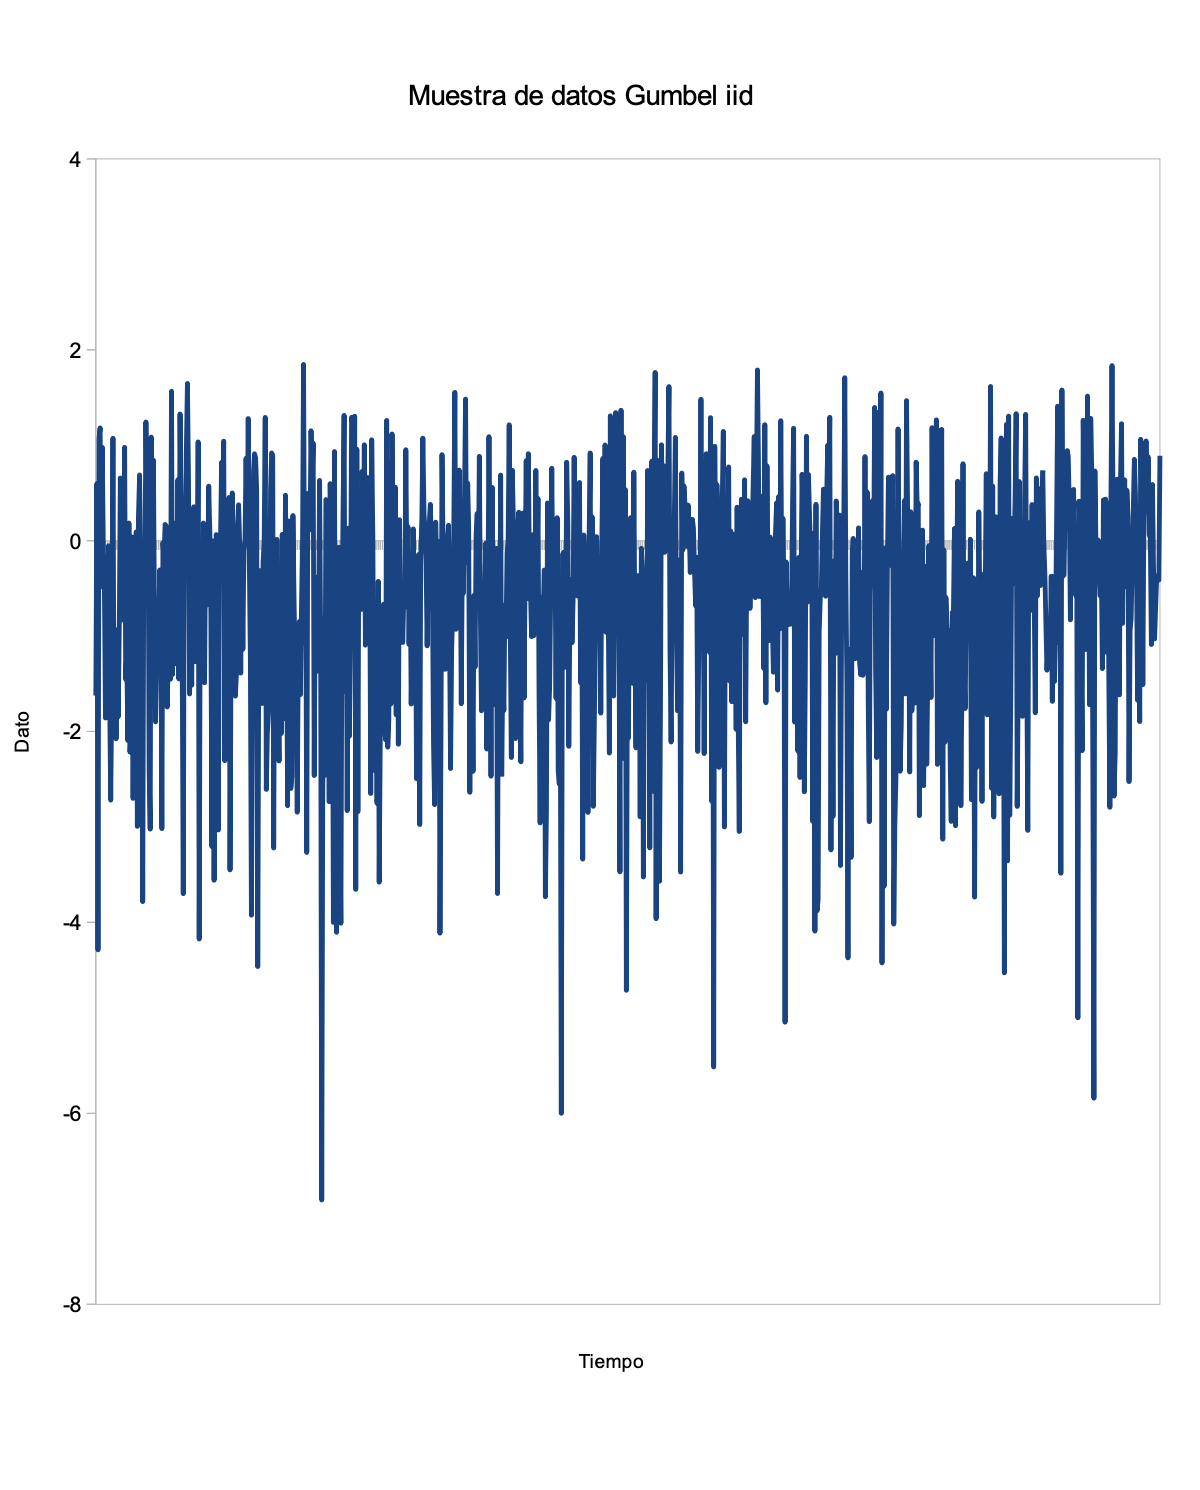
\includegraphics[width=0.9\textwidth,height=\textheight]{images/p1.png}
\caption{Caption for your image}
\end{figure}

Lo más sobresaliente, son las muy bruscas variaciones, que hacen difícil
graficar, variaciones no necesariamente equilibradas respecto a un eje
horizontal, pues la Gumbel es un distribución asimétrica, ``inclinada
hacia la izquierda'', con valor esperado 0,577 pero mediana -0,366; si
se simulara una distribución simétrica como la Normal, se vería mayor
equilibrio entre los picos, etc., pero se podría perder de vista lo
esencial: la oscilación fuerte y que ``el grueso'' de los datos no
parecen tender ni a subir ni a bajar, ni a mostrar ciclos.

Veamos ahora como lucen datos que son Gumbel iid, a los que se les ha
sumado una tendencia parabólica y ciclos sinusoidales.

\begin{figure}
\centering
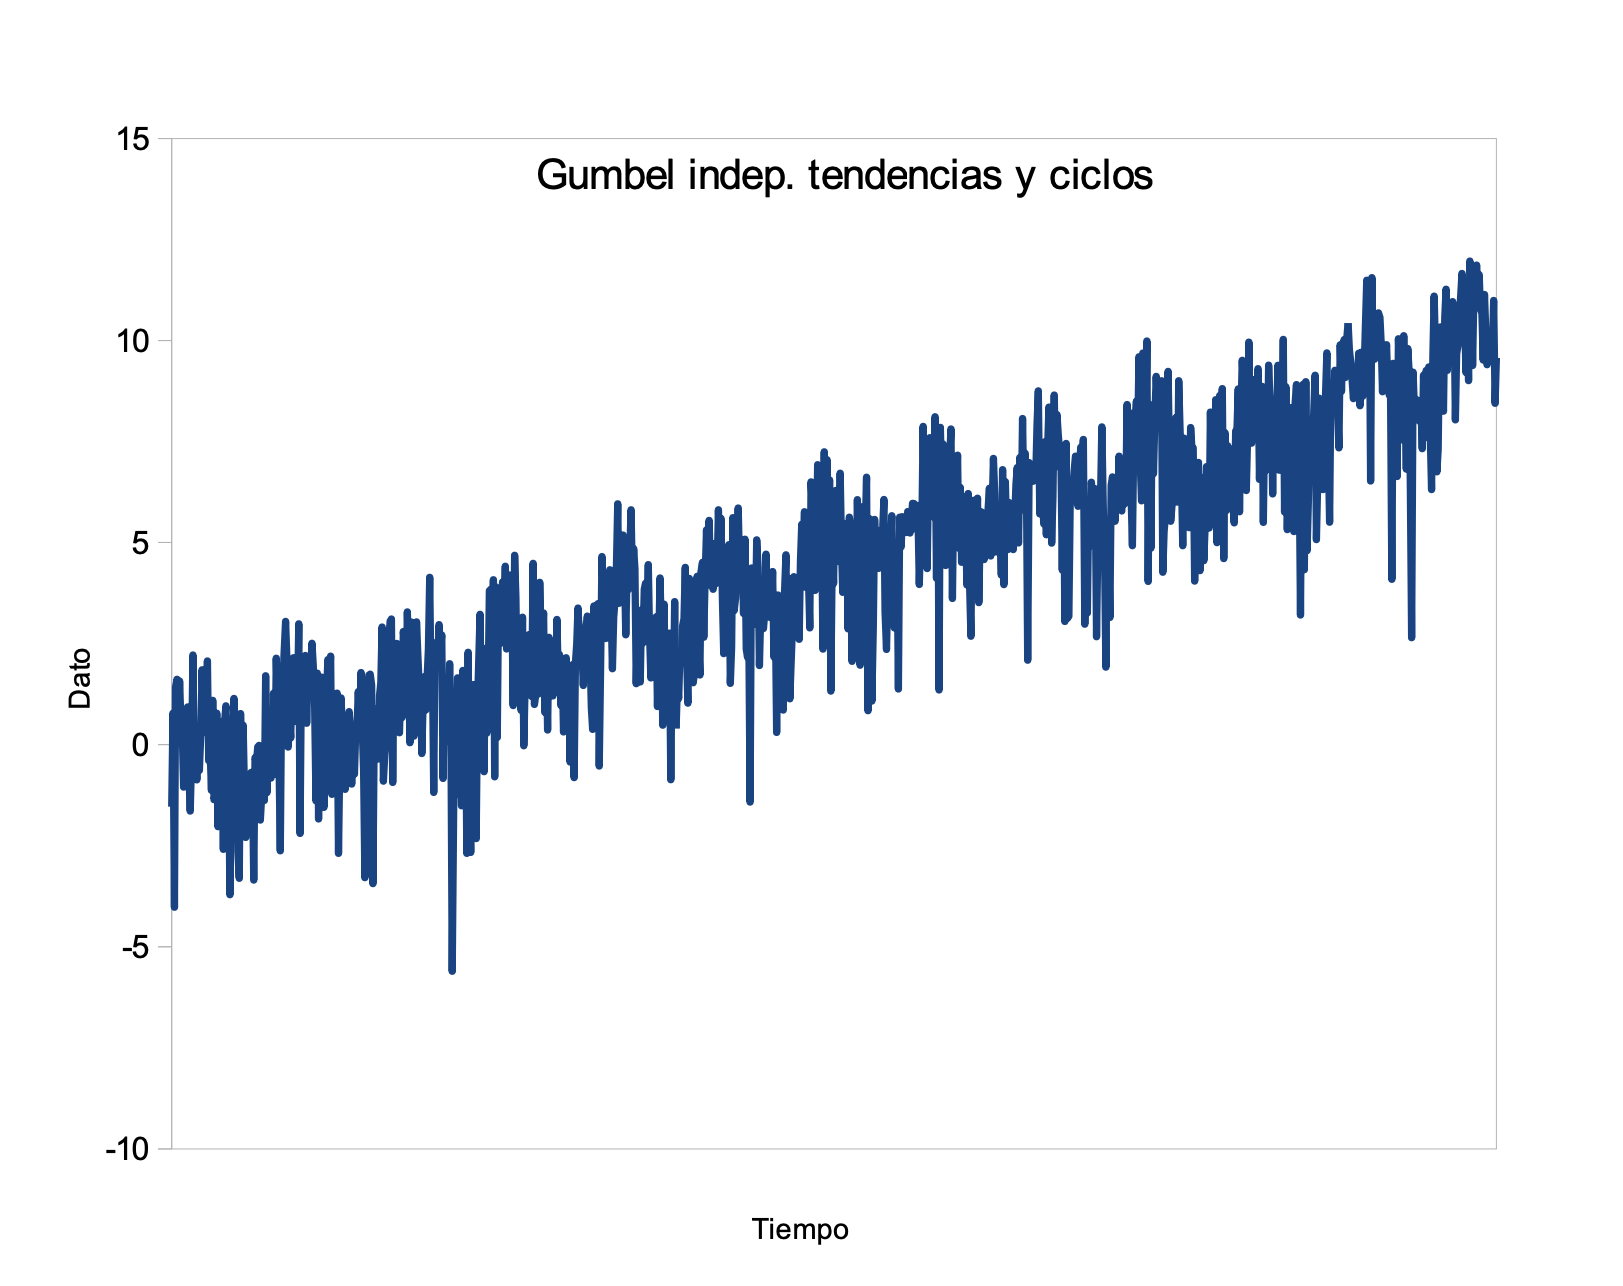
\includegraphics[width=0.9\textwidth,height=\textheight]{images/p2.png}
\caption{Gumbel iid con tendencia parabólica y ciclos sinusoidales.}
\end{figure}

Si bien hay oscilaciones aleatorias, es perceptible a simple vista una
tendencia creciente y la presencia de una estructura cíclica. Tras un
poco de análisis exploratorio uno puede percatarse que la tendencia debe
ser lineal o cuadrática, por lo cual si se propone un polinomio de orden
2 + un término sinusoidal (con parámetros: amplitud, frecuencia y fase),
por mínimos cuadrados se puede ajustar bien, resultando efecrivamente
cuadrática la tendencia. Si se le restara a los datos originales los
valores de las componentes determinísticas (Tendencia+Ciclo) ajustadas,
los nuevos datos que resultan (llamados Residuos) deberían
razonablemente superar los tests para datos iid. Esta es la forma más
sencilla de lidiar con lo no-iid. Veamos ahora la gráfica de
observaciones de un proceso 2-dependiente, estacionario, donde los datos
tienen distribución Gumbel.

Veamos qué pasa ahora si yuxtaponemos la gráfica de Gumbel iid con la de
Gumbel 2-dependiente.

Aún para el ojo más adiestrado es muy difícil distinguir las dos
situaciones. Puede quizás percibirse mayor ``inercia'' en el gráfico
superior, correspondiente a la 2-dependencia, pero es realmente muy
difícil lograrlo (y nada seguro jugarse). Esto demuestra la importancia
de realizar tests de hipótesis sobre la estructura subyacente y no
utilizar el ``ojímetro''. Veamos como luce ahora una serie de datos
Gumbel 2-dependientes con componente cíclica.

Se insinúa una estructura de ciclos, pero nuevamente es altanebte
recomendable chequear la estructura mediante tests. La adición de una
tendencia creciente fuerte, podría ser una técnica exploratoria que
ayudara a visualizar los ciclos, como apuntó Juan Piccini en la primera
edición de este curso. Veamos finalmente como luce la dependencia
fuerte. Nuevamente el proceso es estacionario y los datos son Gumbel.

Las oscilaciones son parecidas a los casos anteriores pero la muy
parejita ``poda'' inferior es la que hace sospechar algo ``raro''. De
todos modos, las posibles estructuras de dependencia fuerte son muchas,
complejas y verificarlas no es sencillo. Como resumen final, en los más
próximos capítulos tomaremos direcciones no iid, en las que veremos:

\begin{enumerate}
\def\labelenumi{\arabic{enumi}.}
\tightlist
\item
  Si el proceso es estacionario y débilmente dependiente, la técnica
  clásica de DEA puede aplicarse esencialmente igual (Leadbetter,
  Lindgren, Rootzén).
\item
  Si el proceso no es estacionario o no es débilmente dependiente,
  cumple algunas propiedades condicionales a otro proceso que le pauta
  la ``fase'', la técnica clásica de DEA puede aplicarse, pero con
  modificaciones no menores. (En realidad veremos en el capítulo 5 un
  trabajo de nuestra co-autoría donde el interés está centrado en el
  punto 2 pero del cual, y como caso particular, surgen resultados para
  el punto 1)
\end{enumerate}

\textbf{Además:} 3.Puede cambiarse el enfoque y mirar el número de
eventos extremos en diversos lapsos, esto lleva en el caso iid a un
proceso de Poisson, para estacionarios y débilmente dependientes a un
Poisson Compuesto y en el marco más general del punto 2, a mezclas de
Procesos de Poisson Compuestos ( Lise Bellanger-GP). El conteo de
eventos extremos será también la base o el ``pie'', para introducir una
técnica muy usada, POT (Picos Sobre Umbrales) y sus variaciones más
recientes que veremos al final.

\newpage

\hypertarget{referencias-bibliogruxe1ficas}{%
\chapter{Referencias
bibliográficas}\label{referencias-bibliogruxe1ficas}}

\vspace{1cm}
\setlength{\parindent}{-0.2in}
\setlength{\leftskip}{0.2in}

\hypertarget{refs}{}
\begin{CSLReferences}{1}{0}
\leavevmode\vadjust pre{\hypertarget{ref-notas_curso}{}}%
Perera, Gonzalo, Angel Segura, y Carolina Crisci. 2021. \emph{Curso de
estadística de datos extremales, cap. 1 a cap. 5}.

\leavevmode\vadjust pre{\hypertarget{ref-evd}{}}%
Stephenson, A. G. 2002. {«evd: Extreme Value Distributions»}. \emph{R
News} 2 (2): 0. \url{https://CRAN.R-project.org/doc/Rnews/}.

\end{CSLReferences}

\backmatter
\end{document}
